\subsection*{1a}
\begin{figure}[h]
    \centering
    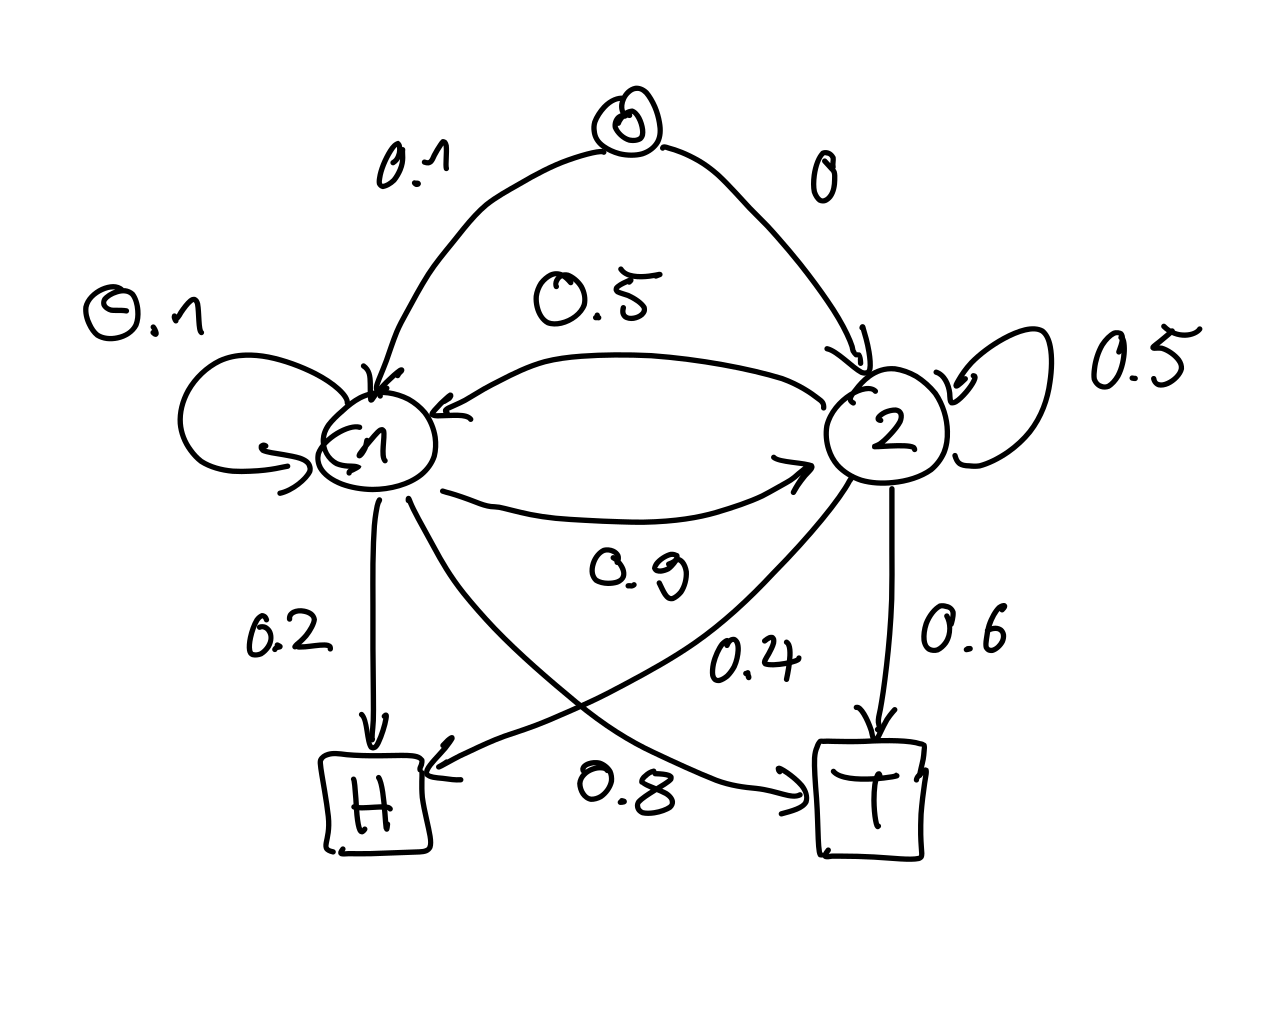
\includegraphics[width=0.8\linewidth]{hmm.png}
    \caption{Name}
    \label{fig:name}
\end{figure}

\subsection*{1b}
We have one coin each for the hidden states in our graph that determines if we change the hidden state or stay with our current hidden state. 
Then we have one visible coin for each hidden state that determines in which visible state we end up.  
That means our experiment starts with one hidden coin. That coin throw determines if we exchange our hidden coin with the other hidden coin. We remember which coin we got.
Based on which hidden coin we currently got we choose our visible coin and throw it to get the next result for our experiment.
After that we can repeat these steps as often as we need to by using our current hidden coin to get the final result. 


\subsection*{1c}

Compute:
\begin{equation}
    P((q_1, q_2 )| (O_1, O_2) = (T, T))
\end{equation}


\begin{align}
    P((q_1, q_2 )| (O_1, O_2) = (T, T)) =
    \frac{P((O_1, O_2) = (T, T) | q_1, q_2) P(q_1, q_2)}
    {P((O_1, O_2) = (T, T))}
\end{align}

Lets first compute $P(q_1, q_2)$:

\begin{center}
\begin{tabular}{c | c | c | c | c}
    $q_1$ & $q_2$ & $P(q_1)$ &  $P(q_2|q_1)$ & $P(q_2| q_1) P(q_1) $\\ \hline
    1       & 1   &   1      &    0.1        &   0.1 \\
    1       & 2   &   1      &    0.9        &   0.9 \\
    2       & 1   &   0      &    -        &   0 \\
    2       & 2   &   0      &    -        &   0 \\
\end{tabular}
\end{center}

Now, we look at $ P((O_1, O_2) = (T, T) | q_1, q_2)$:

\begin{center}
\begin{tabular}{c | c | c | c }
    $q_1$ & $q_2$ & $P(O_1 = T | q_1, q_2)$ & $P(O_2 = T | O_1 = T , q_1, q_2)$ \\ \hline
    1       & 1   & 0.8 & $0.8^2 = 0.64 $\\
    1       & 2   & 0.8 & $0.8 \cdot 0.6 = 0.48$  \\
\end{tabular}
\end{center}

This yields for the numerator $P((O_1, O_2) = (T, T) | q_1, q_2) P(q_1, q_2)$.

\begin{center}
\begin{tabular}{c | c | c }
    $q_1$ & $q_2$ & $P((O_1, O_2) = (T, T) | q_1, q_2) P(q_1, q_2) $ \\ \hline
    1       & 1   & $0.64 \cdot 0.1 = 0.064 $\\
    1       & 2   & $0.48 \cdot 0.9 = 0.432 $  \\
\end{tabular}
\end{center}

If we sum the numerator over $q_1$ and $q_2$, we get the probability of the denominator:
\begin{equation}
    P((O_1, O_2) = (T, T)) = 0.064 + 0.432 = 0.496
\end{equation}

Finally, we can compute the posterior probability $P((q_1, q_2 )| (O_1, O_2) = (T, T))$:
\begin{center}
\begin{tabular}{c | c | c }
    $q_1$ & $q_2$ & $P((q_1, q_2 )| (O_1, O_2) = (T, T))$ \\ \hline
    1       & 1   & $ 0.064 / 0.496 = 4 / 31 $\\
    1       & 2   & $ 0.432 / 0.496 = 27 / 31$ \\
\end{tabular}
\end{center}

